
\documentclass [MS] {uclathes}
\usepackage{amsmath}
\usepackage{booktabs}
\usepackage{graphicx}
\graphicspath{ {./images/} }


% \input {mymacros}                         % personal LaTeX macros

%%%%%%%%%%%%%%%%%%%%%%%%%%%%%%%%%%%%%%%%%%%%%%%%%%%%%%%%%%%%%%%%%%%%%%
%
% Usually things live in separate flies.
%
% \input {prelim}                           % preliminary page info

%%%%%%%%%%%%%%%%%%%%%%%%%%%%%%%%%%%%%%%%%%%%%%%%%%%%%%%%%%%%%%%%%%%%%%%%
%                                                                      %
%                          PRELIMINARY PAGES                           %
%                                                                      %
%%%%%%%%%%%%%%%%%%%%%%%%%%%%%%%%%%%%%%%%%%%%%%%%%%%%%%%%%%%%%%%%%%%%%%%%

\title          {Beating the Book: \\
                A Machine Learning Approach to NBA Win Probabilities \\
                in Search of an Edge Over the Betting Odds}
\author         {Guy Dotan}
\department     {Statistics}
% Note:  degreeyear should be optional, but as of  5-Feb-96
% it seems required or you get a year of ``2''.   -johnh
\degreeyear     {2020}

%%%%%%%%%%%%%%%%%%%%%%%%%%%%%%%%%%%%%%%%%%%%%%%%%%%%%%%%%%%%%%%%%%%%%%%%

\chair          {Frederic R. Paik Schoenberg}
\member         {Vivian Lew}
\member         {Zili Liu}

%%%%%%%%%%%%%%%%%%%%%%%%%%%%%%%%%%%%%%%%%%%%%%%%%%%%%%%%%%%%%%%%%%%%%%%%

%\dedication     {\textsl{To my mother \ldots \\
%                who---among so many other things--- \\
%                saw to it that I learned to touch-type \\
%                while I was still in elementary school}}

%%%%%%%%%%%%%%%%%%%%%%%%%%%%%%%%%%%%%%%%%%%%%%%%%%%%%%%%%%%%%%%%%%%%%%%%

\acknowledgments {(Acknowledgments omitted for brevity.)}

%%%%%%%%%%%%%%%%%%%%%%%%%%%%%%%%%%%%%%%%%%%%%%%%%%%%%%%%%%%%%%%%%%%%%%%%

%\vitaitem   {1974--1975}
%                {Campus computer center ``User Services'' programmer and
%                consultant, Stanford Center for Information Processing,
%                Stanford University, Stanford, California.}
%\vitaitem   {1974--1975}
%                {Programmer, Housing Office, Stanford University.
%                Designed a major software system for assigning
%                students to on-campus housing.
%                With some later improvements, it is still in use.}
%\vitaitem   {1975}
%                {B.S.~(Mathematics) and A.B.~(Music),
%                Stanford University.}
%\vitaitem   {1977}
%                {M.A.~(Music), UCLA, Los Angeles, California.}
%\vitaitem   {1977--1979}
%                {Teaching Assistant, Computer Science Department, UCLA.
%                Taught sections of Engineering 10 (beginning computer
%                programming course) under direction of Professor Leon
%                Levine.
%                During summer 1979, taught a beginning programming
%                course as part of the Freshman Summer Program.}
%\vitaitem   {1979}
%                {M.S.~(Computer Science), UCLA.}
%\vitaitem   {1979--1980}
%                {Teaching Assistant, Computer Science Department, UCLA.}
%\vitaitem   {1980--1981}
%                {Research Assistant, Computer Science Department, UCLA.}
%\vitaitem   {1981--present}
%                {Programmer/Analyst, Computer Science Department, UCLA.}

%%%%%%%%%%%%%%%%%%%%%%%%%%%%%%%%%%%%%%%%%%%%%%%%%%%%%%%%%%%%%%%%%%%%%%%%

%\publication    {\textsl{MADHOUS Reference Manual.}
%                Stanford University, Dean of Student Affairs
%                (Residential Education Division), 1978.
%                Technical documentation for the MADHOUS
%                software system used to assign students to
%                on-campus housing.}

%%%%%%%%%%%%%%%%%%%%%%%%%%%%%%%%%%%%%%%%%%%%%%%%%%%%%%%%%%%%%%%%%%%%%%%%

\abstract       {Lorem ipsum dolor sit amet, consectetur adipiscing elit. Nunc tincidunt dui eros, id tincidunt tellus mattis in. Morbi eget sem nec libero congue ultrices. Mauris dictum enim ut nisl iaculis, eu placerat leo sodales. Nam consectetur fringilla mi et facilisis. Cras egestas nisi eu scelerisque sollicitudin. Etiam sit amet nibh ligula. Aenean euismod tristique ante in eleifend. Mauris nibh nulla, consectetur ac mi ut, tempus suscipit leo. Maecenas vehicula consequat arcu eget feugiat. \\

Donec sed urna nec neque gravida elementum. Nullam turpis odio, venenatis sit amet feugiat dapibus, molestie eget quam. Phasellus justo enim, congue ut risus in, hendrerit posuere nibh. Quisque ultrices euismod pulvinar. Pellentesque eu facilisis libero. Phasellus efficitur porttitor ex vitae aliquam. Morbi metus ipsum, tempor quis lacus sed, interdum tincidunt mauris. Aliquam eget sollicitudin urna. Maecenas et ligula eget nibh maximus finibus. Maecenas justo turpis, rhoncus sit amet posuere at, pulvinar vitae purus. Nunc sed odio dui.}

%%%%%%%%%%%%%%%%%%%%%%%%%%%%%%%%%%%%%%%%%%%%%%%%%%%%%%%%%%%%%%%%%%%%%%%%



\begin {document}
\makeintropages

%%%%%%%%%%%%%%%%%%%%%%%%%%%%%%%%%%%%%%%%%%%%%%%%%%%%%%%%%%%%%%%%%%%%%%
%
% Ordinarily each chapter (at least) is in a separate file.
%
%\input {chapter1}                         % Chapter 1 of dissertation
%\input {chapter2}                         % Chapter 2
%\input {chapter3}                         % etc.
%\input {chapter4}
%\input {chapter5}
%\input {chapter6}
%\input {chapter7}
%\input {chapter8}

%      Chapter 1     %%%%%%%%%%%%%%%%%%%%%%%%%%%%%%%%%%%%%%%%%%%%%%%%%%%%%%%%%%%%
\chapter{Introduction}

\noindent Over the past decade there have been two seminal shifts in the world of sports analytics and consequently the entire professional sports landscape. The first: the proliferation and democratization of accessible data. The second, and more recently: the federal legalization of sports gambling within the United States. \\

\noindent While the sports industry might be one of the newest sectors to be disrupted by the emergence of data-driven decisions challenging preconceived notions from ``experts'', its impact has been fast and far reaching. Setting aside the unprecedented shock to the economic ecosystem---specifically within sports and entertainment---from the 2020 outbreak of COVID-19, the sports analytics business has been thriving. ``The global sports analytics market is expected to reach a revenue of \$4.5 billion by 2024, growing at a CAGR [Compound Annual Growth Rate] of 43.5\%'' [1]. \\

\section{Current State of Sports Analytics}
\noindent To the general public, the most well-known adoption of analytics into the sports universe was within Major League Baseball, thanks largely to Michael Lewis' 2003 book \emph{Moneyball} and subsequent movie blockbuster, staring Brad Pitt, in 2011. This story, which chronicles the influence of Bill James, the field of empirical baseball research known as Sabermetrics, and the story of the 2002 Oakland A's success has been the poster child of how data can create a competitive edge on the playing field. But sports analytics has made its impression in far more avenues than just baseball. The field is responsible for the increased emphasis of the three-point shot in basketball, the use of optical player tracking technology in the NFL, and even the statistical optimization of curling game strategy that led the Swedish women's national team to a gold medal in the 2018 Winter Olympics [2], just to name a few. \\

\noindent The integration of data analysts and scientists as a crucial element of professional sports organizations appears here to stay, but the acceleration in the field's adoption can be tied to the increased availability of data. The NFL and NBA hold yearly hackathons to allow anyone the opportunity to dive into their sport's data and present findings to top league officials with prizes and networking at stake. Conferences such as Sloan Sports Analytics Conference in Boston began as a small gathering of about 100 attendees in 2006, and now in 2020, attracts over 4,000 people. The conference has gained national recognition, notably hosting former President Barack Obama as the keynote speaker in 2018. The industry's explosion in popularity, though, has been aided by communities such as FiveThirtyEight, Retrosheet, Sports-Reference, and league-offered APIs bestowing data democracy to anyone that desires. Sports analytics has largely become open-source and this hivemind has benefited players, teams, and organizations. \\

 \section{The Legalization of Sports Gambling}
\noindent On May 14, 2018, the Supreme Court case \emph{Murphy v. National Collegiate Athletic Association} reached a landmark decision regarding the federal government's right to control a state's ability to sponsor sports betting. In a 6-3 decision, the Professional and Amateur Sports Protection Act of 1992 (PASPA) was overturned, thus opening the doors for every state to make its own laws permitting in-state sports wagering. \\

\noindent In just two years since the ruling there are already 17 states with full-scale legalization and another five that have passed legislation that will take effect in the coming year. [3] And as one would expect, bettors in legal states have flocked to sportsbooks, both digital and brick-and-mortar. (Sportsbooks, or ``books'', are places, often times part of a greater casino, where bettors can make wagers on all types of sporting events.) Since the overturning of PASPA, Americans have placed over \$20 billion of bets which has generated \$1.4 billion of revenue in those legal states. [4] Morgan Stanley projects that in just five years, by 2025, almost three-quarters of US states (36) will have legalized sports betting and the U.S. market could see \$7 to \$8 billion in revenue. [5] \\

\begin{figure}[h]
\centering
  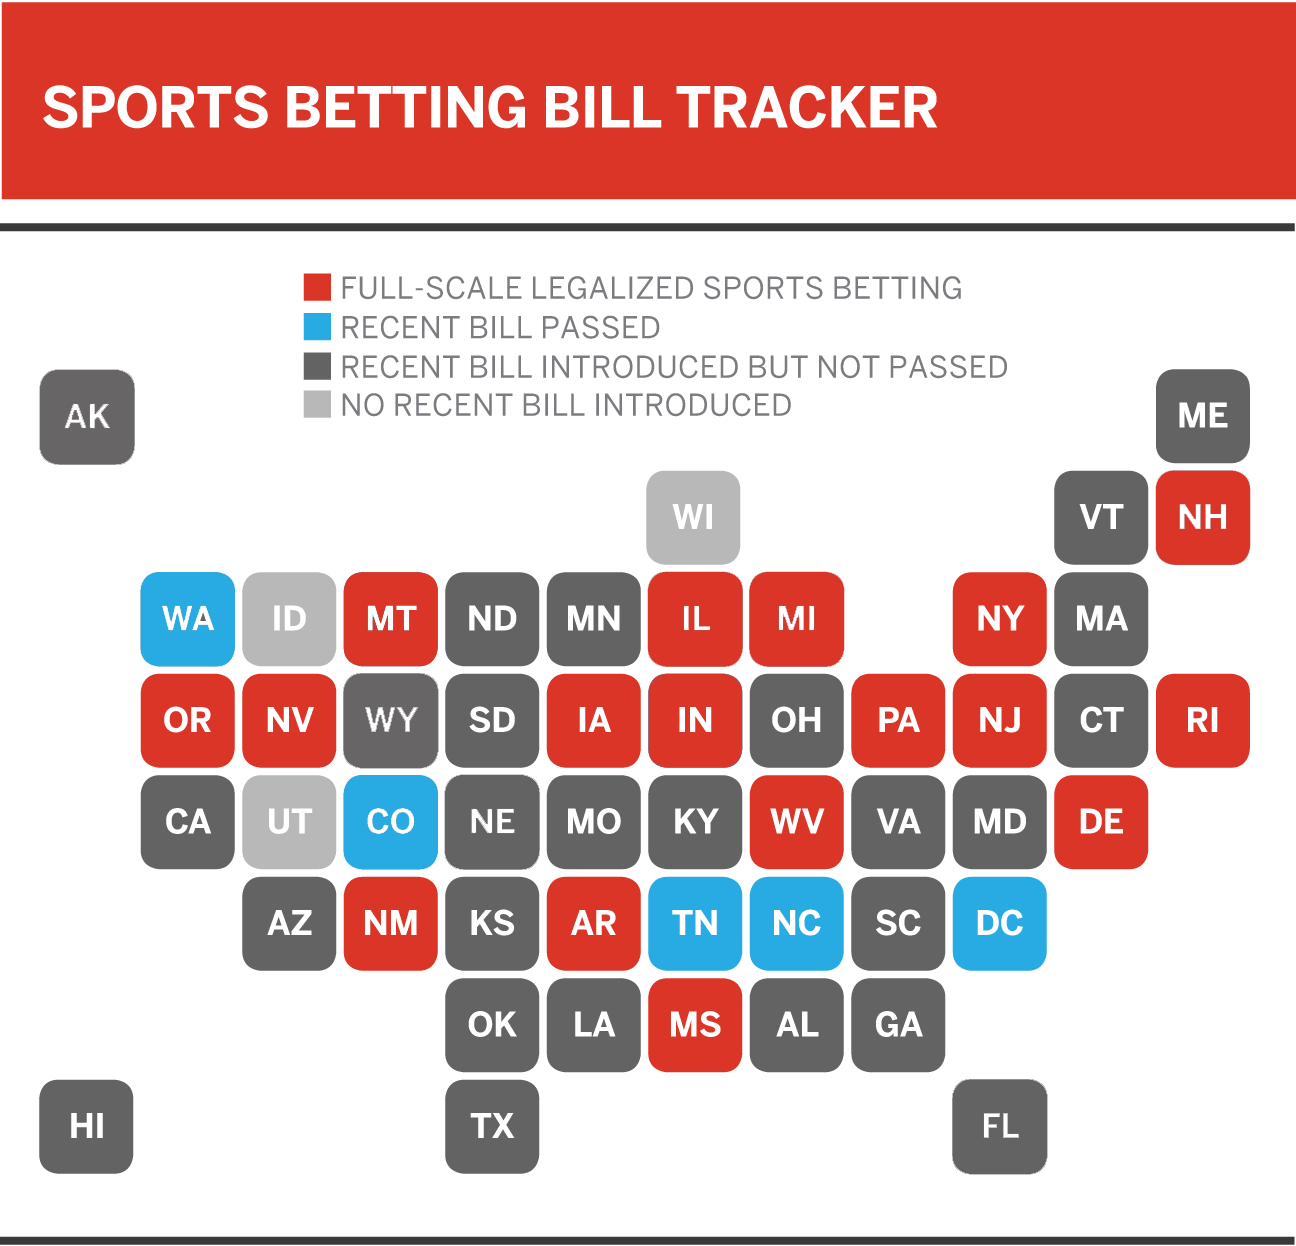
\includegraphics[width=250px]{20200326_betting_map.png}
  \caption{U.S. map of the current state of sports gambling legislation (as of March 2020)}
\end{figure}

\section{The Intersection of Data and Wagering}
\noindent Sportsbook operators within casinos have had decades of experience building a complex infrastructure of analytics to help them determine where to set up their gambling lines. Their goal is to set up a bet every game such that there is an even amount of money wagered on both sides of the bet. This allows them to take their cut of the wagers (known in the industry as the ``vigorish'' or ``vig'') and thus drive revenue to their casino, no matter which team wins. For the entirety of their existence, sportsbooks have maintained a significant edge over the majority of bettors. Their advantage was largely based on their access to data and domain expertise building models to determine how to establish the perfect betting line. It is this statistical edge that has keeps income flowing into the sportsbooks within casinos. Money that helps build lavish 50-story casinos and hotels that makes Las Vegas strip world-renowned. That said, surprisingly, sports wagering makes just 3\% of gaming revenue in Nevada casinos. \\

\begin{figure}[h]
\centering
  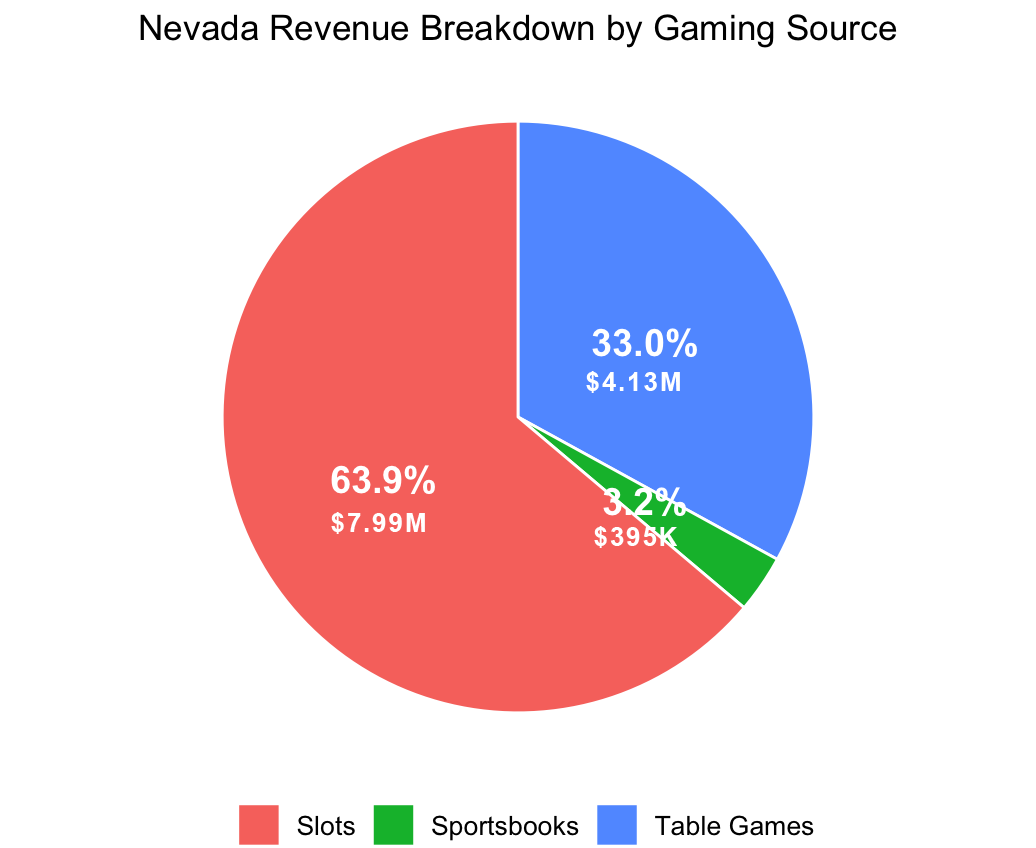
\includegraphics[width=300px]{gaming_revenue.png}
  \caption{Total gaming revenue by source in Nevada from Mar. 1, 2019 to Feb. 29, 2020 [6]}
\end{figure}

\noindent But now, with sports wagering becoming more commonplace in the American society and the proliferation of available sports data to everyday consumers, there is an opportunity to close the gap between casinos and bettors. Similar to how stockbrokers use proprietary projection models to systematically ``beat the market'', sports wagering has followed suit. \\

\noindent Recall, a sportsbook's objective on each bet is to account for an even amount of money wagered on both sides. Often times a betting line is skewed by the inherent biases of an average sports bettor. For example, if the Los Angeles Lakers (a TV market size of over five million people) were to play the San Antonio Spurs (TV market size of just 900 thousand), we might expect a sportsbook to make a line that slightly favors the Spurs. Even if the teams were evenly matched, sportsbooks would expect a disproportionate amount of hometown favorite bets supporting the Lakers. Just the smallest marginal edge, demonstrated by this example, could be enough to be exploited by an adept model. A model, when applied to a large enough dataset, could yield a considerate return on investment. \\

\noindent The goal of this study is to determine if applying machine learning methods to vast sports datasets (in this case, within the NBA) can create such a model that would give a bettor the competitive edge over the lines set by a sportsbook. \\


%      Chapter 2     %%%%%%%%%%%%%%%%%%%%%%%%%%%%%%%%%%%%%%%%%%%%%%%%%%%%%%%%%%%%
\chapter{The Mathematics of Sports Gambling}

\noindent In order to understand how to beat the bookmakers, one first needs to understand how to interpret the betting lines they provide. There is a wide array of different types of bets that a person can make at a sportsbook. The three most popular betting styles are: ``point spreads'', ``over/unders'', and ``moneylines''. The following are descriptions of these types of bets using basketball as an example.\\

\section{Point Spreads, Over/Unders, and Moneylines}
Point spreads are mechanisms used to account for the discrepancy between two unevenly matched teams. Usually noted by: Warriors (-5) vs. Clippers or the inverse: Clippers (+5) vs. Warriors. The number in the parenthesis is called the ``spread.'' Essentially, the sportsbook believes that the Warriors are more likely to win the game, but the book wants to drive an even amount of bettors to wager on the Clippers (even though they are underdogs) as the Warriors. Therefore, their bookmakers suggest placing a spread of five points on the game. So, if I bet on the Warriors they need to win by more than 5 points for me to win the bet. If I bet on the Clippers, they have to lose by 4 points or fewer or win the game, for me to cash in on the wager. If the game ends with the Warriors winning by 5 points, then this is called a ``push'' and all bettors get their money back. Sometimes a spread will be listed at 0 points (called a ``pick-em''), indicating that this is an even matchup and all you have to do is pick the winner to win the bet.\\

\noindent Similar to point spreads, over/unders involve a specific point amount that a bettor needs to wager on the correct side of. However, in this case, the winner of the game is irrelevant. All the bettor must do is guess if the combined score between the teams will be greater than or less than the over/under line. For example, Warriors vs. Clippers (+200). If I bet the ``over 200'', I am expecting the combined score between the two teams to reach 201 or more and it does not matter what combination in occurs (Warriors 120-Clippers 81, Clippers 101-Warriors 100, etc.) If the final combined score is exactly 200, again this is called a push and bettors get their money back. For this reason, over/unders (and spreads for that matter), oftentimes use fractional lines (+5.5 or +200.5) to prevent the case of a push. Over/unders can be offered for single quarters, just the first half, just the second half, or even for a single team's score.\\

\noindent The third type of popular betting type are called moneylines and are the relevant bet type for this study. In a moneyline bet, a person simply needs to determine which team will win the game. But if one team was heavy favorite versus the other team, it would not make sense for a sportsbook to pay out and an equal amount for choosing the favorite as choosing the underdog. As a result, sportsbooks offer a moneyline, which adjusts the amount you win for having your bet hit based on the likelihood that team will win the game. Moneylines are notated in various formats: decimal, fractional, and moneyline. The first two are commonly used in Europe. This paper will use the moneyline odds notation since they are most common to the US (and often called ``American'' odds). Moneylines are written as follows: Warriors (-235) vs. Clippers, or conversely, Clippers (+185) vs. Warriors. \\

\noindent Essentially, these either positive or negative, three-digit numbers, imply how much money a bettor would profit relative to a \$100 bet. +185 means that if a bettor laid \$100 on the Clippers, and then they won the game, the bettor would make \$185 profit. -235 means that a bettor would have to wager \$235 in order to profit \$100 from that game. So if a bettor placed \$100 on the Warriors at -235 moneyline odds, and the Warriors indeed won, the bettor makes \$42.55 profit. 

\noindent \text{\underline{Moneyline Profit - Underdog}} \\
\text{Let $Profit_{dog} = \Pi_{d}$ } \\
\begin{equation} \label{ml_prof_dog}
\begin{split}
\frac{ML}{100}  & = \frac{\Pi_{d}}{Risk}  \\
100*\Pi_{d} & = ML*Risk    \\
\Pi_{d} & = \frac{ML}{100} * Risk 
\end{split}
\end{equation}

\noindent \text{Using our example...}
\begin{equation*} 
\begin{split}
\Pi_{d} & = \frac{+185}{100} * 100 \\
 & = 1.85 * 100 \\
 & = \$185
\end{split}
\end{equation*}


\noindent \text{\underline{Moneyline Profit - Favorite}} \\
\text{Let $Profit_{fav} = \Pi_{f}$ } \\
\begin{equation} \label{ml_prof_fav}
\begin{split}
\frac{-1 * ML}{100}  & = \frac{Risk}{\Pi_{f}}  \\
\Pi_{f} * (-1 * ML) & = Risk * 100  \\
\Pi_{f} & = \frac{100}{(-1 * ML)} * Risk 
\end{split}
\end{equation}

\noindent \text{Using our example...}
\begin{equation*} 
\begin{split}
\Pi_{f} & =  \frac{100}{(-1 * -235)} * 100 \\
 & = \frac{100}{235} * 100 \\
 & = .4255 * 100 \\
 & = \$42.55
\end{split}
\end{equation*}

\noindent In summary, a \$100 bet on the Clippers (+185) leads to \$185 profit. A \$100 bet on the Warriors (-235) leads to about \$42 profit. This discrepancy in profits is to discourage enough bettors from taking the favorite Warriors and instead take the potential for upside in profit by betting on the underdog Clippers. Again, the sportsbooks goal is to optimize these moneylines to set it at a line such that an even amount of money is placed on both sides. \\

\section{Implied Win Probability}
The payout formula for moneylines makes it quite simple to determine how much profit a bettor can make from having their wager hit. Risk averse bettors tend to take favorites (negative moneylines) despite the lower payouts because there is a higher chance that the team they bet on will win. Risky bettors will seek out underdogs with lower probabilities of winning, but they think will actually surprise the public, win the game, and thus provide a larger profit-margin. \\

\noindent In addition to the payout, however, moneylines can actually be converted into a win probability known as ``implied probability''. The implied probability formula is defined as the size of the bettor's wager divided by the return on investment for that wager. Or simply: risk over return.

\begin{equation} \label{imp_prob}
\begin{split}
& Implied Probability = \frac{Risk}{Return}  \\
\end{split}
\end{equation}
Note: \emph{Return} = \emph{Risk} + \emph{Profit}

\section{Derivation of Implied Win Probability}
A universal formula to calculate the implied win probability for any bet (underdog or favorite) can be derived by plugging in the formula for moneyline profit for an underdog (equation \ref{ml_prof_dog}) and a favorite (equation \ref{ml_prof_fav}) into the implied formula (equation \ref{imp_prob}).

\noindent \text{\underline{Implied Probability - Underdog}} \\
\begin{equation} \label{ip_dog}
\begin{split}
IP_{dog} & = \frac{Risk}{Return}  \\
& = \frac{Risk}{Risk + \Pi_{d}}  \\
& = \frac{Risk}{Risk + \left( \frac{ML}{100}*Risk \right)} \\ 
& = \frac{Risk}{Risk \left( 1 + \frac{ML}{100}  \right)} \\ 
& = \frac{1}{ 1 + \frac{ML}{100} } \\ 
IP_{dog} & = \frac{100}{100 + ML} 
\end{split}
\end{equation}


\noindent \text{\underline{Implied Probability - Favorite}} \\
\begin{equation} \label{ip_dog}
\begin{split}
IP_{dog} & = \frac{Risk}{Return}  \\
& = \frac{Risk}{Risk + \Pi_{f}}  \\
& = \frac{Risk}{Risk + \left( \frac{100}{-1 * ML} \right) * Risk } \\ 
& = \frac{Risk}{Risk \left( 1 + \frac{100}{-1 * ML}  \right)} \\ 
& = \frac{1}{ 1 + \frac{100}{(-1 * ML)} } \\ 
IP_{dog} & = \frac{(-1 * ML)}{(-1 * ML) + 100} 
\end{split}
\end{equation}

\noindent \text{\underline{Implied Probability - General Equation}} \\
\[
IP(ML) =
\begin{cases}
\displaystyle
 \frac{100}
 {ML * 100},  & \text{if ML} \geq 0 \\ \\ 
\displaystyle
 \frac{(-1 * ML)}
 {(-1 * ML) +100}, &  \text{if ML} <  0\\ 
\end{cases}
\]

\section{The Vig or the Juice}
As mentioned previously, the goal of a sportsbook is to have an equal amount of money placed on both sides of a wager so that no matter the results, they will make money once they take their cut of the bets. This cut is known as the vigorish, and more colloquially, the ``vig'' or the ``juice.'' So how does one calculate the juice? Let's use our example from above with the Warriors versus the Clippers. \\

\noindent The Warriors moneyline odds were -235, which after using the derived formula, comes out to an implied probability of 70.15\%. The Clippers moneyline odds were +185 and therefore an implied probability of 35.09\%. Now the most basic rule of probability states that the sum of all possible probabilities of an event always equals 1. And more specifically, the probability of an event plus the probability of the complement of that event equals 1. If we consider the chances that a team wins a game as the probability while the chances they lose is the complement of that probability, we would expect these two events to sum to 1. See below: \\ 

\noindent \text{\underline{Given:}} \\
\noindent \text{$P(A) + P(A^{c}) = 1 $ } \\
\noindent \text{Let ...} \\
\noindent \text{$P(A)$ =  Probability that Warriors win } \\
\noindent \text{$P(A^{c})$ = Probability that Warriors lose (i.e. Clippers win)} \\
\noindent \text{$P(A)$ =  0.70 } \\
\noindent \text{$P(A^{c})$ =  0.35 }
\begin{flalign*}
P(A) + P(A^{c}) & =  &&\\
0.70 + 0.35 & = 1.05 &&\\ 
1.05 & \neq 1
\end{flalign*}

\noindent So these two implied probabilities are mutually exclusive, compose the entire space of outcomes, and yet sum to over 100\%. This summed probability (in this case 105\%) that is greater than 1 is called the ``overround'' and is how sportsbooks take their cut. By setting the betting lines such that the probabilities result in an overround, the sportsbook effectively ensures that they will gain a profit from this wager. In our example above, a \$100 bet on the Warriors pays out \$42, while a \$100 bet on the Clippers pays out \$185. In order to determine how much a sportsbook would expect to pay out from these implied probabilities can be calculated as follows:

\noindent \text{\underline{Expected Profit:}} \\
\noindent \text{Let $E(\Pi) $ = Expected Profit for Sportsbook} \\
\noindent \text{$E(\Pi_i) = \Pi_i * P(win_i) $ } \\
\noindent \text{ $E(\Pi) = \sum_i{\Big( E(\Pi_{i}) \Big) } $} \\
\noindent \text{ $E(\Pi) = \sum_i{\Big( \Pi_i * P(win_i) \Big) } $} \\
\noindent \text{ $E(\Pi) = \Pi_A * P(win_A) + \Pi_{A^C} * P(win_{A^C}) $} \\

\noindent \text{Using our example...} \\
\noindent \text{$E(\Pi_A) $ = Expected Profit if Warriors Win} \\
\noindent \text{$E(\Pi_{A})  = \Pi_{A} * P(A)$} \\
\noindent \text{$E(\Pi_A) $ = \$42 * 0.7 = $\sim$\$30} \\
\noindent \text{$E(\Pi_{A^C}) $ = Expected Profit if Clippers Win} \\
\noindent \text{$E(\Pi_{A^C})  = \Pi_{A^C} * P(A^C)$} \\
\noindent \text{$E(\Pi_{A^C}) $ = \$185 * 0.35 = $\sim$\$65} \\
\noindent \text{$E(\Pi)$ = \$30 + \$65 } \\
\noindent \text{= $\sim$\$95} \\


\noindent As seen above, this overround (105\%) of the probabilities creates the vig for the casino. If the sportsbook were to take \$100 of total wagers on this bet, on average, they would expect to pay out just \$95. Thus, ensuring a cut of about \$5 for this wager. Now consider the fact that casinos collect millions of dollars on bets, not \$100, it is easy to see why sports gambling is such a lucrative endeavor for bookkeepers, especially when the optimal moneylines are established (and therefore the juice is optimized as well). \\

\section{``Removing the Juice'' - Actual Win Probability}
In order to get a clear idea of the sportsbooks' expectations of how likely each of the two teams is to win a matchup, we need to get rid of the guaranteed profit they bake into the lines. The implied probabilities are derived from the betting lines, but the actual probabilities are what remains after taking the vig into account. Probability theory claims that the sum of all possible events in a sample space should always equate to 1. So to get the true probabilities based on the betting odds, the implied probabilities need to be skewed so that they also sum to 1. The method to remove the vig is simple, just divide the probability by the overround. \\

$$
\displaystyle
Actual Probability = \frac{Implied Probability}
{Overround}
$$

$$
\text{Actual Probability the Warriors Win} = \frac{70\%}{105\%} = 67\% \\
$$
$$
\text{Actual Probability the Clippers Win} = \frac{35\%}{105\%} = 33\% \\
$$

We see that the two probabilities now sum up to 100\% and therefore represent the true probability that the sportsbook places on each team's chances of winning. In summary: \\

\begin{table}[ht!]
\resizebox{\textwidth}{!}{%
\begin{tabular}{@{}lrrrrrr@{}}
\toprule
Team     & \multicolumn{1}{l}{Moneyline Odds} & \multicolumn{1}{l}{Risk} & \multicolumn{1}{l}{Profit} & \multicolumn{1}{l}{Return} & \multicolumn{1}{l}{Implied Win Probability} & \multicolumn{1}{l}{Actual Win Probability} \\ \midrule
Warriors & -235                               & \$100                    & \$42                       & \$142                      & 70\%                                        & 67\%                                       \\
Clippers & +185                               & \$100                    & \$185                      & \$285                      & 35\%                                        & 33\%                                       \\ \bottomrule
\end{tabular}%
}
\caption{Summary of betting values for sample wager}
\label{tab:bet-summary-table}
\end{table}



%      Chapter 3     %%%%%%%%%%%%%%%%%%%%%%%%%%%%%%%%%%%%%%%%%%%%%%%%%%%%%%%%%%%%
\chapter{Exploratory Analysis}

%      Chapter 4     %%%%%%%%%%%%%%%%%%%%%%%%%%%%%%%%%%%%%%%%%%%%%%%%%%%%%%%%%%%%
\chapter{Random Forest}

%      Chapter 5     %%%%%%%%%%%%%%%%%%%%%%%%%%%%%%%%%%%%%%%%%%%%%%%%%%%%%%%%%%%%
\chapter{Neural Network}

%      Chapter 6     %%%%%%%%%%%%%%%%%%%%%%%%%%%%%%%%%%%%%%%%%%%%%%%%%%%%%%%%%%%%
\chapter{Betting Results}

%      Chapter 7    %%%%%%%%%%%%%%%%%%%%%%%%%%%%%%%%%%%%%%%%%%%%%%%%%%%%%%%%%%%%
\chapter{Kelly Criterion}

%      Chapter 8     %%%%%%%%%%%%%%%%%%%%%%%%%%%%%%%%%%%%%%%%%%%%%%%%%%%%%%%%%%%%
\chapter{Conclusions}


%\bibliography {bib/network,bib/naming}    % bibliography references
%\bibliographystyle {thesis}

\end {document}

